% Author: Magdalen Berns

\chapter{The Physiology of The Eye}

\label{anatomy}
\lhead{\emph{The Physiology of The Eye}}
\section{A Normal, Healthy Eye}
\label{anatomy}

The cornea is a transparent layer around 0.6mm thick, which curves over
the iris of the eye over its anterior chamber.
\cite{yaylali1997corneal,thoft1983x,patel1994refractive}
With a mean refractive index of around 1.4 (about the same as water),
the cornea allows plenty of light to pass through, but refracts as a
convergent lens due to its convex, shape. \Eref{eq:refractive} shows
Snell's Law of refraction for a light wave passing through two different
isotropic materials which have refractive indices $n_1$
and $n_2$, respectively.

\begin{figure}[htbp]
  \centering
    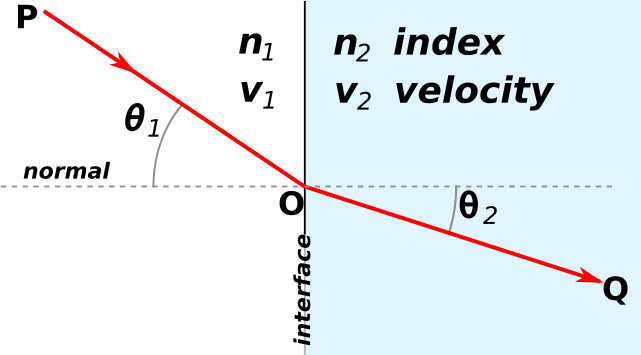
\includegraphics{figures/snells}
  \caption{Snell's law for diffraction at an interface where $n_1$ \textless $n_2$}
  \label{fig:snell}
\end{figure}

The angle $\theta_1$ is normal to the boundary between $n_1$ and $n_2$
and the angle $\theta_2$ is normal to the boundary between $n_2$ and $n_1$
as shown in \fref{fig:snell}

\begin{equation}
n_1\sin\theta_1=n_2\sin\theta_2
\label{eq:refractive}
\end{equation}

The radius of the human cornea tends to decrease with age and the cornea
itself, takes on a more spherical shape.\cite{guirao2000optical} Its
outermost surface is made of epithelial cells which are continuously lost
and replaced.\cite{jester1999cellular,hassell2010molecular} The reproduction
of cells is facilitated in part by tear ducts, which  serve to moisten the
eyes and remove harmful bacteria.\cite{holly1977tear}

There is a small circular opening in the iris, (the coloured section of
the eye) the pupil, has an aperture which dilates to allow an appropriate
amount of refracted light to pass through the lens. Light is refracted
once again through the lens converges towards a focal point on the back
of the eye. The lens makers expression in \eref{eq:lens_makers} is an
expression described by the diagram in \fref{fig:convergent_lens} which
shows light passing through a convex lens for calculating the focal point,
$f$ of distances $S_1$ and $S_2$ either side of a given convex lens.
\cite{greivenkamp2004field}

\begin{equation}
\frac{1}{S_1} + \frac{1}{S_2} = \frac{1}{f}
\label{eq:lens_makers}
\end{equation}

\begin{figure}[htbp]
  \centering
    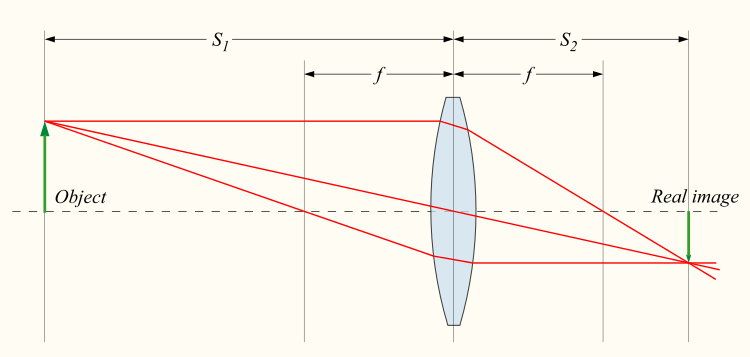
\includegraphics{figures/convergent_lens2}
  \caption{light passing through a convex lens for calculating the focal
  point, $f$ of distances $S_1$ and $S_2$ either side of a given convex lens.}
  \label{fig:convergent_lens}
\end{figure}

A ciliary body of tissue made up of fiber and muscle which accommodates the
lens and secretes a fluid, known as Aqueous Humour into a canal that flows
around the circumference of the eye called the Scleral Venous Sinus.
\cite{bill1970effects,dvorak1934schlemm}

When it becomes necessary to focus on objects at short distances, the
ciliary body muscles contract and suspensory ligaments attached to the
posterior chamber and the posterior lens to become taut, causing the
lens to become somewhat flatter, in response to applied contractile
forces.\todo{some physics here?} When objects are far away the light
is more parallel to the lens' principle axis, the muscles relax and
suspensory ligaments attached to the posterior chamber and the posterior
lens so that it is no longer being accommodated so it can take on a more
rounded shape.

Photons of light are refracted out of the lens, before they pass through
a clear substance called the vitreous chamber and land onto the retina,
which is also transparent. A diagram which identifies the optic axis
and visual axis is shown in \fref{fig:optic_axis}.

\begin{figure}[htbp]
  \centering
    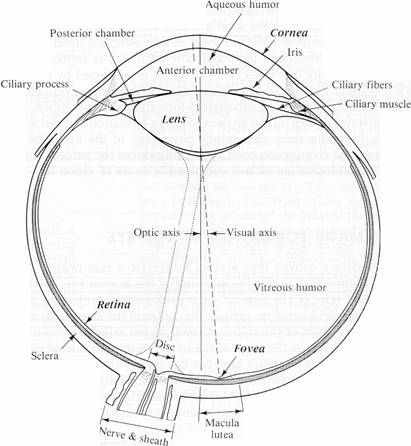
\includegraphics{figures/eye_diagram}
  \caption{A diagram of the eye which includes a visualisation of the visual
   and optic axis, the cornea, the retina and the fovea}
  \label{fig:optic_axis}
\end{figure}

The retina is a membrane which covers the entire receptive field of vision,
it is part of the central nervous system.\cite{rogers1983neurite} Just behind
the retina are ganglion cells, biploar cells, cones and rods. These are supported
by pigment epithelium cells and the coroid, a vascular bed of tissues which
supplies the retina with blood and removes toxins.\cite{lutty1996localization}

There are around 0.7 to 1.5 million ganglion cells in a normal human retina.
\cite{curcio1990topography}. Retinal ganglion cells are  they are part of
the system which passes electrical signals to the brain.
\cite{meyer1995characterization} A diagram of the retinal [something] system
is shown in \todo{figure}

Cones and rods are photoreceptors that ensure that light is converted into
electrical signals \todo{rephrase} and sent to the brain. These signals can
be transmitted to the brain via bunches of ganglion nerves.

Whilst cones are not particularly sensitive to light, they do aid to visual
acuity by granting us colour vision.\cite{bowmaker1980visual} Conversely, cones
which have a region of pigments around $1\mu{m}$, are particularly sensitive,
even to single the pressure exerted by single photons of light at a time,
so they tend to be located around the periphery of the receptive field of
the retina.\cite{liebman1964sensitive,baylor1979responses}

Most of the retinal cones are located around a circular trough in the
receptive field, called the fovea centralis which is located at the center
of the macular.\cite{hendrickson1994primate} The fovea has an apparent dip
because unlike the periphery, there are neurons situated behind it, Neurons
have axons that allow electrical signals travel to the optic nerve so they
can be interpreted by the brain but as the fovea is a particularly sensitive
aid to colour vision and acuity, axons of neurons would get in the way if
they were located directly behind it.

A healthy and normal eye will pick up the full spectrum of colours.
\fref{fig:wavelengths} shows normalised absorbency against wavelength
for red, green and blue cones and rods (which cannot differentiate
between colours), in an average, human eye.

\begin{figure}[htbp]
  \centering
    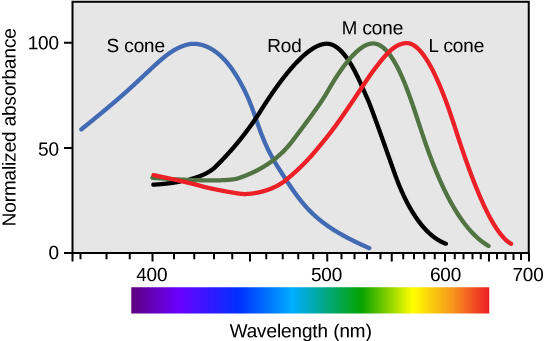
\includegraphics{wavelengths}
  \caption{Normalised absorbency vs. wavelength, for an average eye.}
  \label{fig:wavelengths}
\end{figure}

\section{Development and Dysfunction}

During the early stages of development in babies, there is a steady
increase of a lubricating substance called glycosaminoglycan hexosamine,
in the cornea which reaches an increase plateau at around 2 years of age.
\cite{praus1975glycosaminoglycans}

\todo[inline]{link these two paragraphs}

Some men are born with limited functionality in cones which are
sensitive to particular frequencies of light.\cite{george1996clinical}
If all the eye cones are not working then this causes blindness
to occur but if only some types of cones have limited functionality
as photoreceptors this causes a less serious impairment, commonly
referred to as "colour blindness".

\section{Ageing and Disease}

As humans age, ciliary muscles weaken and this impairs the ciliary
muscles' ability to accommodate the lens and the result of this is
difficulty focusing on objects which are close by.\cite{fisher1985ciliary}

\todo[inline]{link these two paragraphs}

Macular degeneration of pigment cells and decreases in Equatorial rods
and ganglion cell rates is also a common problem for the aged.
\cite{gao1992aging} Preliminary studies show that the thickness
of the coroid decreases with age, but little is understood about
how this may affect vision. \cite{margolis2009pilot} However, it is
widely understood by researchers that age related macular degeneration
can be serious enough to lead to blindness.\cite{klein2005complement}
